% Overview:
%   Benchmarking TeX subfile for the project.
%   Each subfile MUST start with the following line
%		\documentclass[../main.tex]{subfiles}

\documentclass[../main.tex]{subfiles}

\begin{document}

\section{Benchmarking dei Framework}

In questa sezione verranno fatte alcune considerazioni rispetto alle prestazioni dei framework analizzati nelle sezioni precedenti e in particolare, ove possibile, essi verranno direttamente confrontati fra loro. Abbiamo già sottolineato nelle relativa analisi, che, in generale, i metodi \textit{alignment-free} sono in grado di ottenere prestazioni temporali molto inferiori ai metodi che si basano sull'allineamento, velocizzando il processo di genotipizzazione, anche se, in alcuni casi, l'utilizzo di memoria viene incrementato. \textcolor{red}{qui bisogna aggiungere cose, forse considerazioni singole o non so, ne parliamo. Poi vedi se rispetto a discosnp++ nel confronto sotto vuoi fare altre considerazioni}\\


\cite{bernardini2019malva} presentano i risultati di un loro esperimento \footnote{L'esperimento è stato eseguito su un sistema Linux a 64 bit (Kernel 4.4.0) dotato di quattro processori Intel Xeon a 8 core da 2,30 GHz e 256 GB di RAM.} su un dataset reale \footnote{Il dataset utilizzato è IlluminaWGS, individuo NA12878, \textit{coverage} 30x (Zook et al., 2014, Integrating human sequence data sets provides a resource of benchmark SNP and indel genotype calls.). Come genoma di riferimento viene usato GRCh37 e per il set di varianti note, i file VCF forniti dalla Fase 3 di 1KGP che contengono  84 739 838 varianti, le informazioni genotipiche di 2 504 individui e la frequenza a priori di ciascun allele di ciascuna variante.} che compara MALVA con VarGeno \cite{sun-medvedev2018vargeno}, DiscoSnp\texttt{++} \cite{peterlongo2017discosnp++} e due pipeline basate sull'allineamento, BCFtools (Li, 2011, A statistical framework for SNP calling, mutation discovery, association mapping and population genetical parameter estimation from sequencing data.) e GATK (McKenna et al., 2010, The genome analysis toolkit: a mapreduce framework for analyzing next-generation DNA sequencing data.). Il test viene suddiviso in due parti, \texttt{FullGenome} utilizzando l'intero dataset e \texttt{HalfGenome} con circa la metà delle varianti e le read del dataset.


Ogni metodo è stato valutato in termini di accuratezza ed efficienza (tempo e memoria) della chiamata delle varianti. Le due seguenti Figure \ref{fig:confronto1} e \ref{fig:confronto2} rappresentano graficamente le prestazioni ottenute.

\begin{figure}[h!]
\centering
\begin{minipage}{.5\textwidth}
  \centering
  \captionsetup{justification=centering}
  \vspace*{0,9cm}
  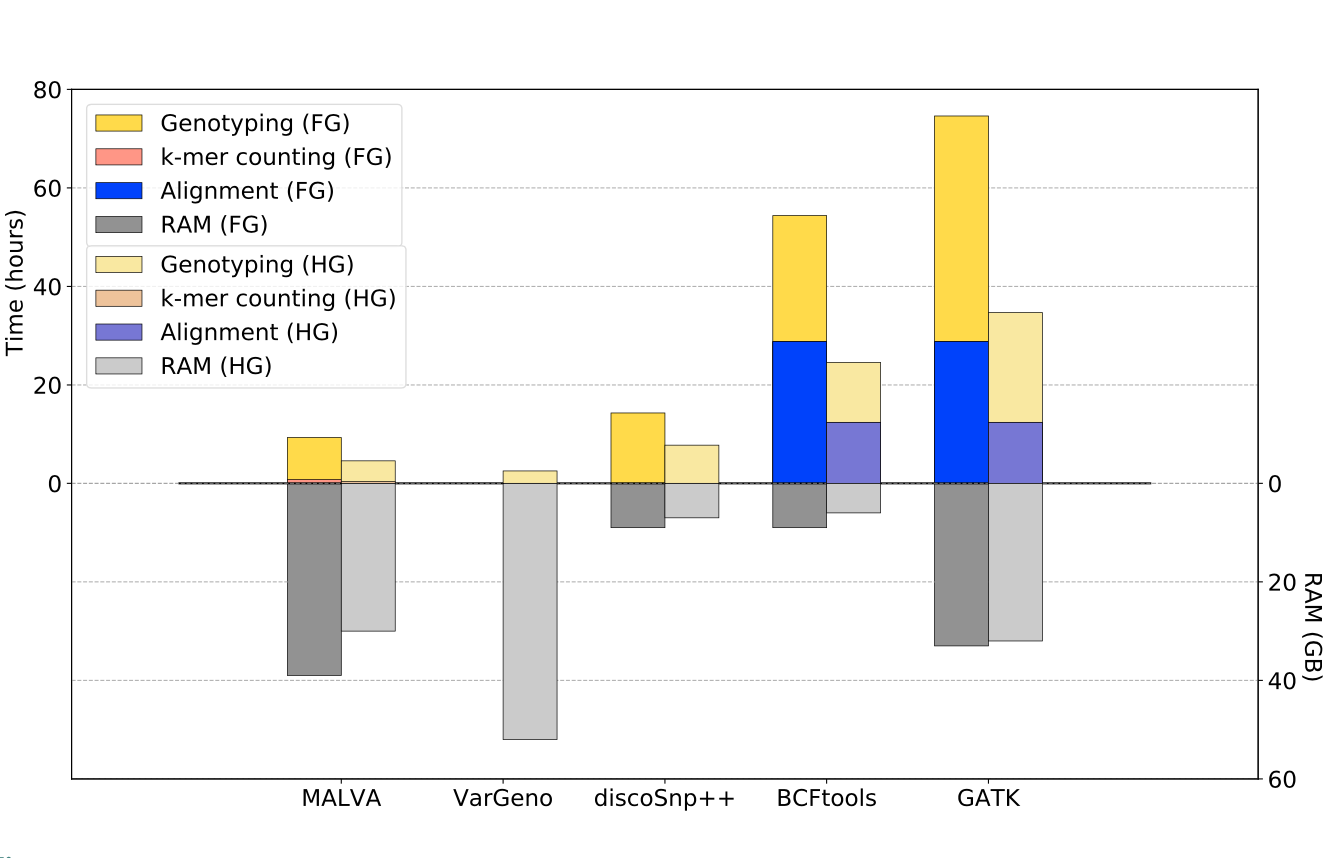
\includegraphics[scale=.39]{images/confronto1.png}
  \captionof{figure}{Tempo di esecuzione e utilizzo della memoria rispetto all'intero dataset \texttt{FullGenome}(FG, prima colonna) e a \texttt{HalfGenome}(HG, seconda colonna).}
  \label{fig:confronto1}
\end{minipage}%
\begin{minipage}{.5\textwidth}
  \centering
  \captionsetup{justification=centering}
  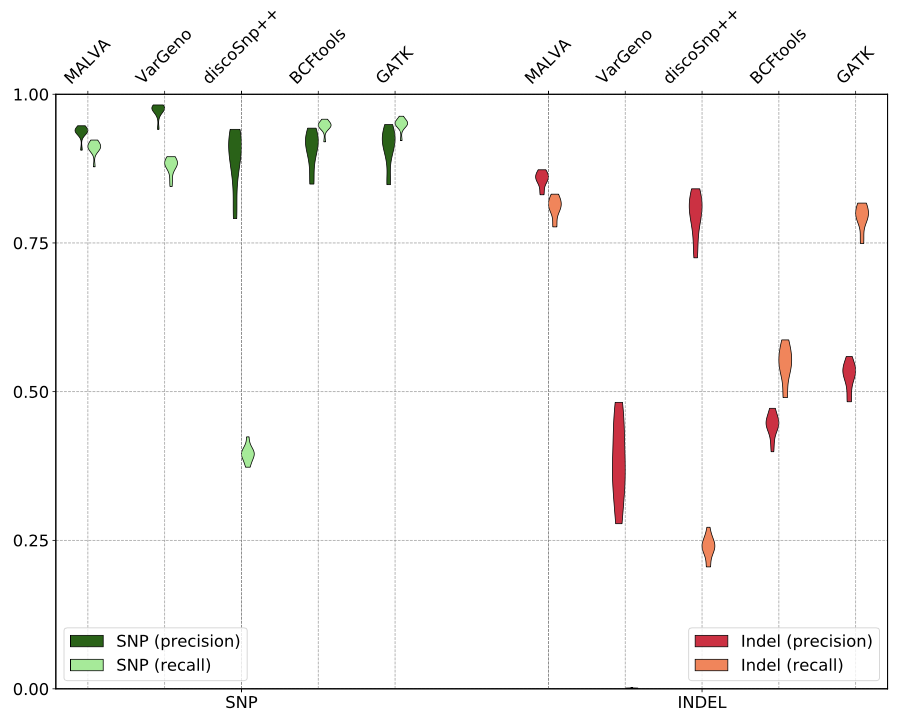
\includegraphics[scale=.50]{images/confronto2.png}
  \captionof{figure}{Rappresentazione qualitativa dell'accurancy rispetto a \texttt{HalfGenome} dataset.}
  \label{fig:confronto2}
\end{minipage}
\end{figure}


Come previsto, MALVA, VarGeno e DiscoSnp\texttt{++} sono più veloci (rispettivamente 4.5, 2.5 e 7.5 ore) dei due approcci basati sull'allineamento testati (24.5 e 34.5 ore) che spendono molto tempo per l'allineamento.


Rispetto all'utilizzo di memoria, tra i tool \textit{mapping-free} DiscoSnp\texttt{++} si è rivelato l'approccio meno dispendioso, seguito da MALVA che aumenta il consumo di memoria di solo il 23\% per il dataset più grande. VarGeno invece richiede molta memoria, come già dichiarato nella relativa sezione: a causa della troppa memoria richiesta, non è stato possibile per gli autori completare il test sull'intero dataset, mentre per il dataset \texttt{HalfGenome} è stato utilizzato quasi il doppio di quella richiesta da MALVA nello stesso dataset.


La precisione e il richiamo di tutti gli strumenti sono relativamente elevate e comparabili: riportiamo delle considerazioni sul test con \texttt{HalfGenome} per poter confrontare anche VarGeno. VarGeno ottiene la miglior precisione sulle chiamate di SNP (97.5\%) rispetto a MALVA (93.8\%) e DiscoSnp\texttt{++} (89.5\%); questo perchè VarGeno preferisce non chiamare SNP in caso di incertezza mentre MALVA, per evitare la perdita di qualsiasi informazione potenzialmente interessante, preferisce rilevare qualsiasi potenziale allele alternato, a scapito di una leggera perdita di precisione. DiscoSnp\texttt{++} presenta il richiamo più basso (39.3\%) in confronto a MALVA (91.1\%) e VarGeno (88.1\%).


Sugli indel, MALVA ha ottenuto precisione e richiamo migliori rispetto agli altri tool. Come previsto, poiché VarGeno non è progettato per gestire gli indel, è stato in grado di genotipizzarne solo una bassa percentuale. DiscoSnp\texttt{++} invece, ha raggiunto un'alta precisione ma è stato in grado di chiamare solo meno di un quarto degli indel totali (24.2\%). I tool basati sull'allineamento hanno una bassa precisione rispetto agli indel, dovuta principalmente alle difficoltà di allineamento delle read che si sovrappongono agli indel. Analizzando inoltre la dimensione degli indel, MALVA si è rivelato l'unico strumento in grado di chiamare indel lunghi (oltre $\sim$40/50 basi), mentre gli altri strumenti sono limitati a indel brevi (che sono anche i più comuni): in ogni caso MALVA ha prestazioni migliori anche sugli indel corti, confermando di aver raggiunto l'obiettivo prefissato e di essere in grado di genotipizzare SNP multi-allelici e indel.\\


\textcolor{red}{Non lo so se basta la prima parte o se inserire anche questo, in caso affermativo commento la tabella. Dimmi tu}
Inoltre, \cite{bernardini2019malva} effettuano un confronto più approfondito tra MALVA e VarGeno (\ref{fig:confronto3}); gli indel non sono stati inclusi nell'analisi.

\begin{figure}[h!]
	\centering
  	\captionsetup{justification=centering}
  	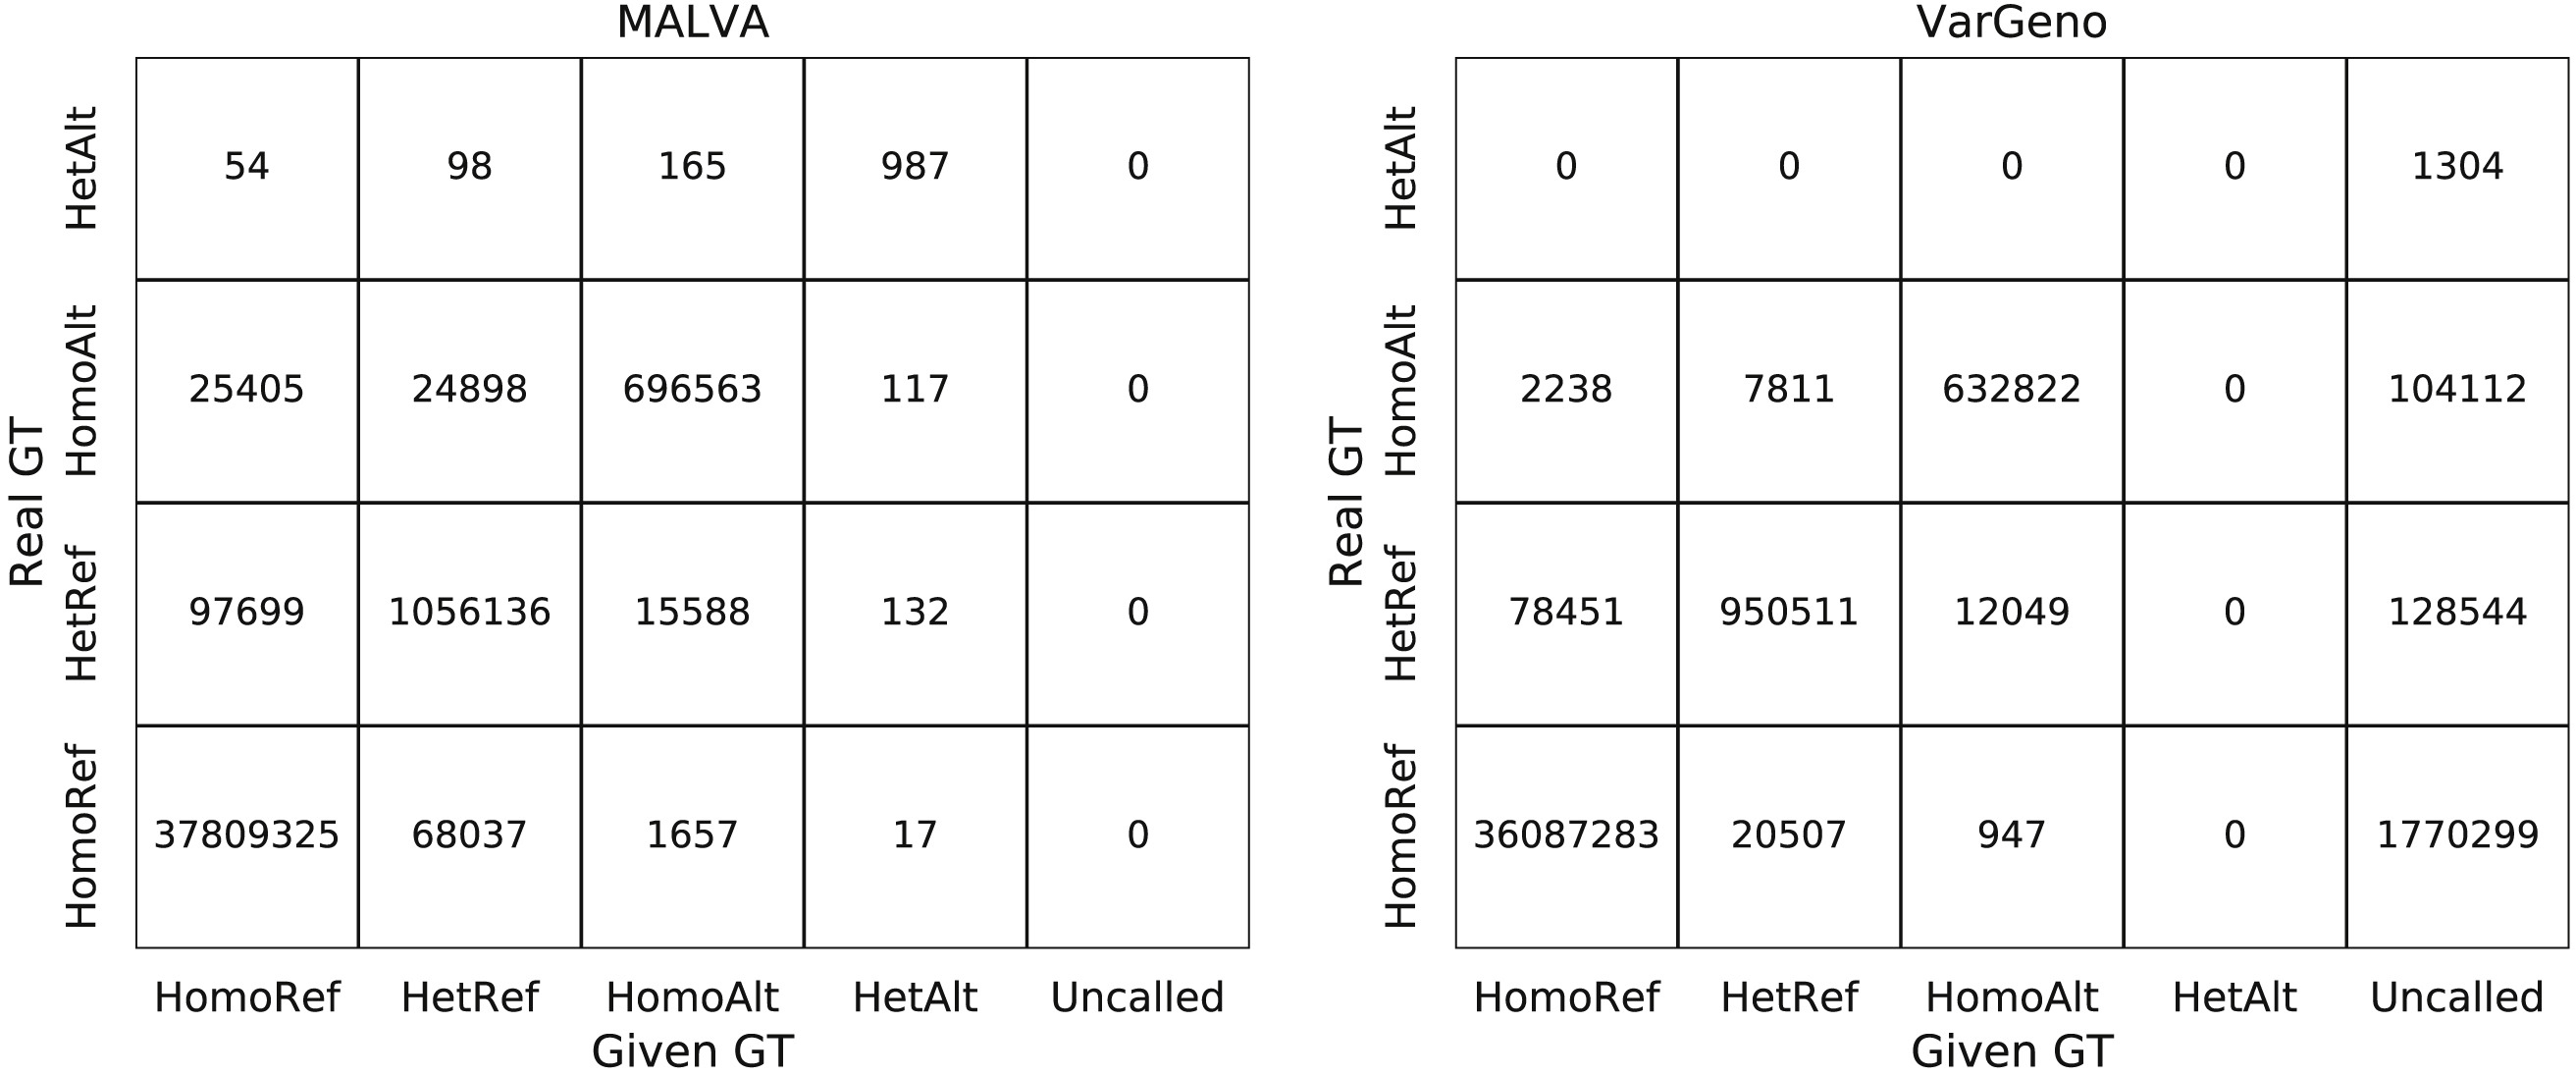
\includegraphics{images/confronto3.jpg}
  	\caption{Confronto tra genotipi reali (dataset 1000 Genome Project) e chiamati da MALVA e Vargeno.}
  	\label{fig:confronto3}
\end{figure}


Per i due metodi viene riportato il numero di output di genotipi corretti, raggruppandoli in riferimento omozigote (HomoRef), riferimento eterozigote (HetRef), alternato omozigote (HomoAlt) e alternati eterozigoti (HetAlt). 



























\end{document}
